\documentclass[11pt]{article}

\usepackage[margin=1in]{geometry}
\usepackage{amsmath,amssymb,amsthm}
\usepackage{mathtools}
\usepackage{bm}
\usepackage{hyperref}
\usepackage{graphicx}
\usepackage{xcolor}
\usepackage{booktabs}
\usepackage{enumitem}
\usepackage{float}
\usepackage{caption}
\usepackage{subcaption}

\newcommand{\dg}{^{\dagger}}
\newcommand{\Ng}{N_{g}}
\newcommand{\dV}{\Delta V}

\title{gGA Dimer Scans: $U/t$ Dependence at $\dV=0$ and $\dV=2$\\
\large (Ghost Multiplicities $\Ng=2$ and $\Ng=4$, Direct-Minimization Solver)}
\author{gGut\_mau project --- \texttt{not\_imp\_gga\_dimer.py}}
\date{\today}

\begin{document}
\maketitle
\tableofcontents

\bigskip
\noindent\textbf{Scope.} This note collects the $U/t$ scans produced by the
direct-minimization (``not\_imp'') gGA solver for the half-filled Hubbard dimer,
at zero and finite site-splitting potential $\dV$ (see \texttt{not\_impurity.tex}
for the solver's equations and \texttt{code.tex} for the $\dV$ generalization).
Four scans are collected:
\begin{itemize}[nosep]
  \item \texttt{scan\_ng2\_not\_imp} --- $\Ng=2$, $\dV=0$;
  \item \texttt{scan\_ng4\_not\_imp} --- $\Ng=4$, $\dV=0$;
  \item \texttt{scan\_ng2\_dV2\_confirmed} --- $\Ng=2$, $\dV=2$, cross-checked
        against the impurity-problem solver;
  \item \texttt{scan\_ng4\_dV2\_confirmed} --- $\Ng=4$, $\dV=2$, cross-checked
        against the impurity-problem solver.
\end{itemize}
All scans sweep $U/t \in [0.1,\,10.0]$ in steps of $0.1$, at $t=1$. The
``confirmed'' scans report the lowest-energy solution after reconciling the two
independently implemented solvers (impurity-problem and direct-minimization);
see commit \texttt{fe06bd6}.

%=====================================================================
\section{\texorpdfstring{$\Ng=2$}{Ng=2}}
\label{sec:ng2}

\subsection{Total energy vs. \texorpdfstring{$U/t$}{U/t}}

Figure~\ref{fig:ng2_E} shows the variational ground-state energy $E_{\rm var}/t$
as a function of $U/t$, at $\dV=0$ and $\dV=2$.

\begin{figure}[H]
  \centering
  \begin{subfigure}[b]{0.48\textwidth}
    \centering
    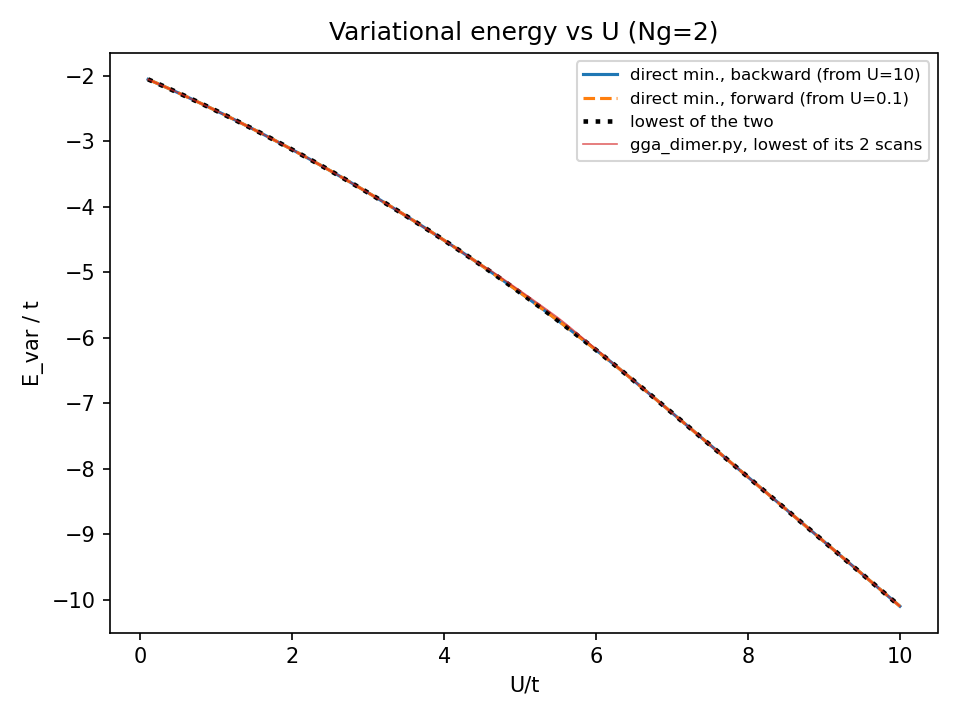
\includegraphics[width=\textwidth]{../scan_ng2_not_imp/E_vs_U.png}
    \caption{$\dV=0$}
  \end{subfigure}
  \hfill
  \begin{subfigure}[b]{0.48\textwidth}
    \centering
    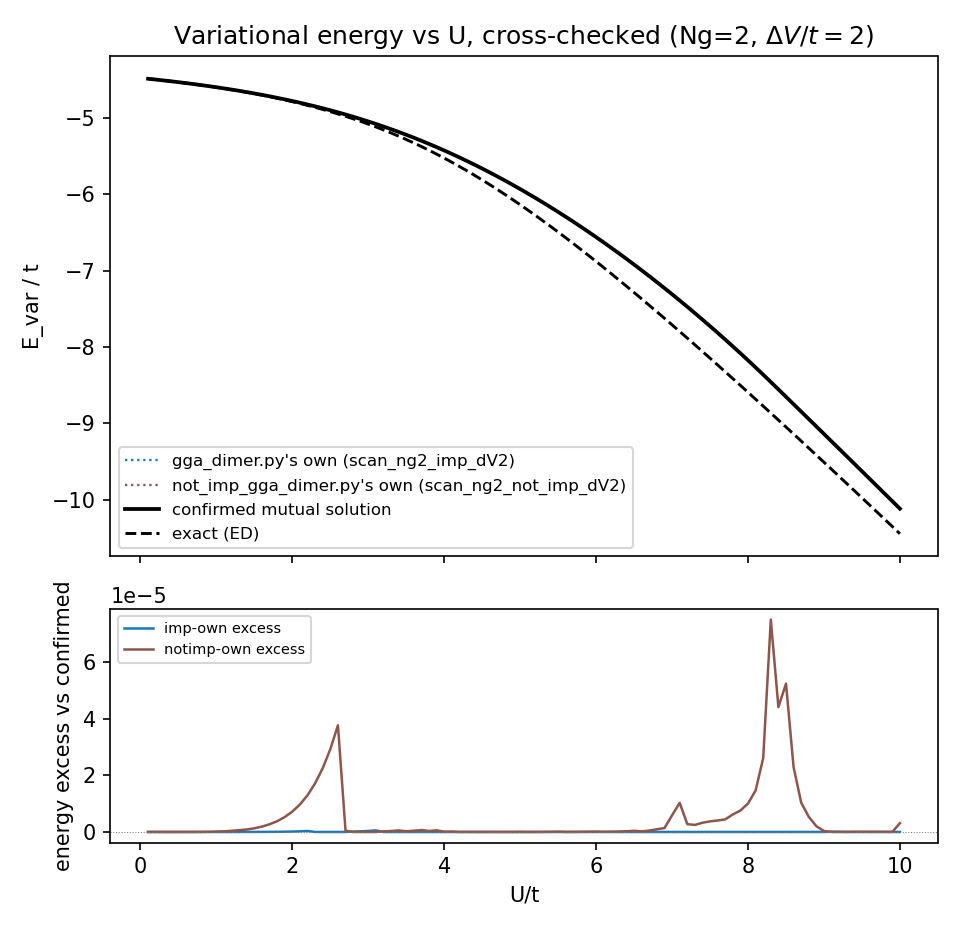
\includegraphics[width=\textwidth]{../scan_ng2_dV2_confirmed/E_vs_U.png}
    \caption{$\dV=2$}
  \end{subfigure}
  \caption{$\Ng=2$: total energy $E_{\rm var}/t$ vs. $U/t$.}
  \label{fig:ng2_E}
\end{figure}

\subsection{Quasiparticle spectrum: 3D view}

Figure~\ref{fig:ng2_3d} shows the full quasiparticle energy spectrum
$\{\epsilon^{qp}_n\}$ as a function of $U/t$ (ridgeline / 3D representation).

\begin{figure}[H]
  \centering
  \begin{subfigure}[b]{0.48\textwidth}
    \centering
    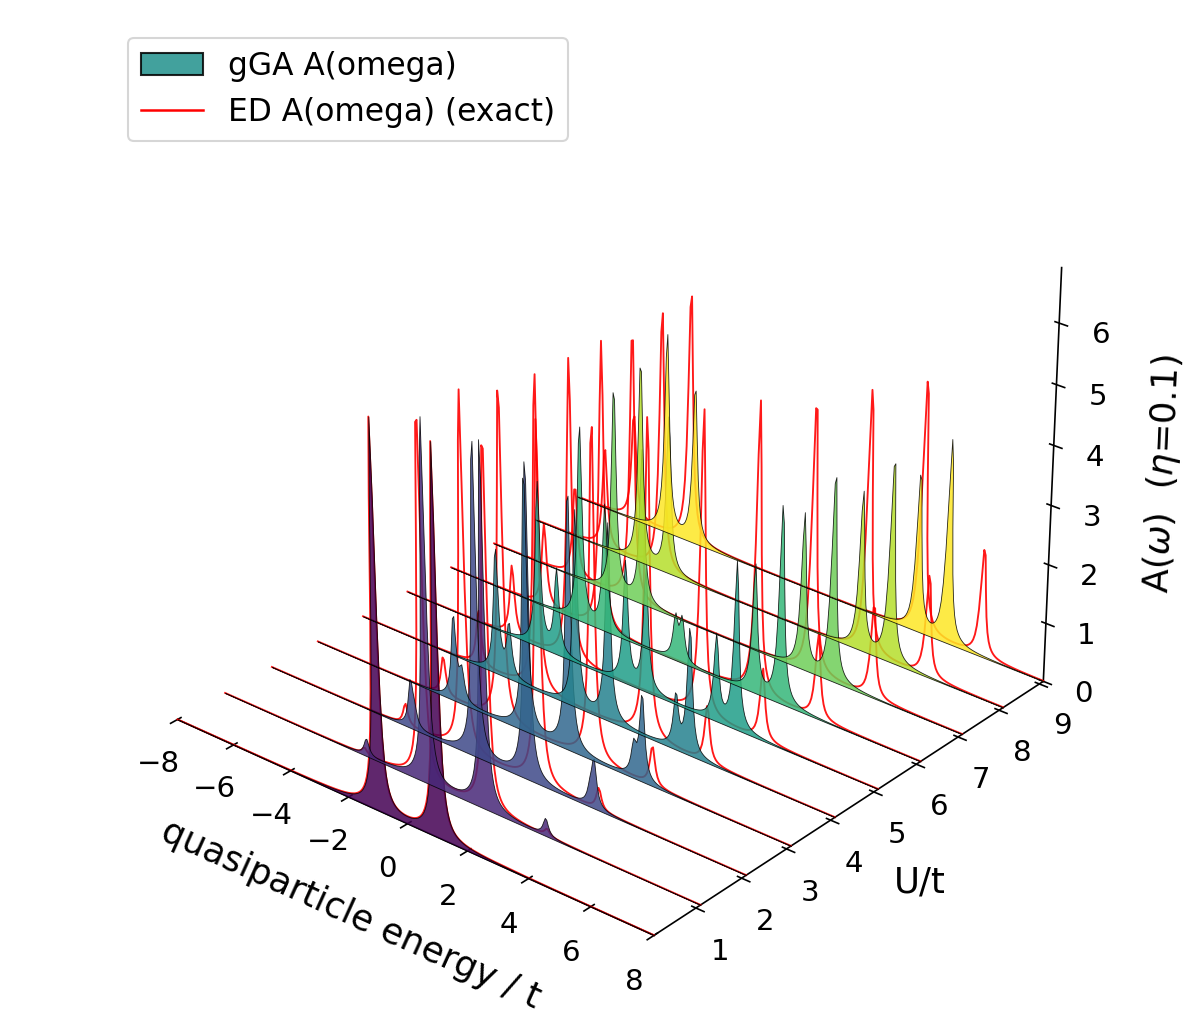
\includegraphics[width=\textwidth]{../scan_ng2_not_imp/eqp_vs_U_3d.png}
    \caption{$\dV=0$}
  \end{subfigure}
  \hfill
  \begin{subfigure}[b]{0.48\textwidth}
    \centering
    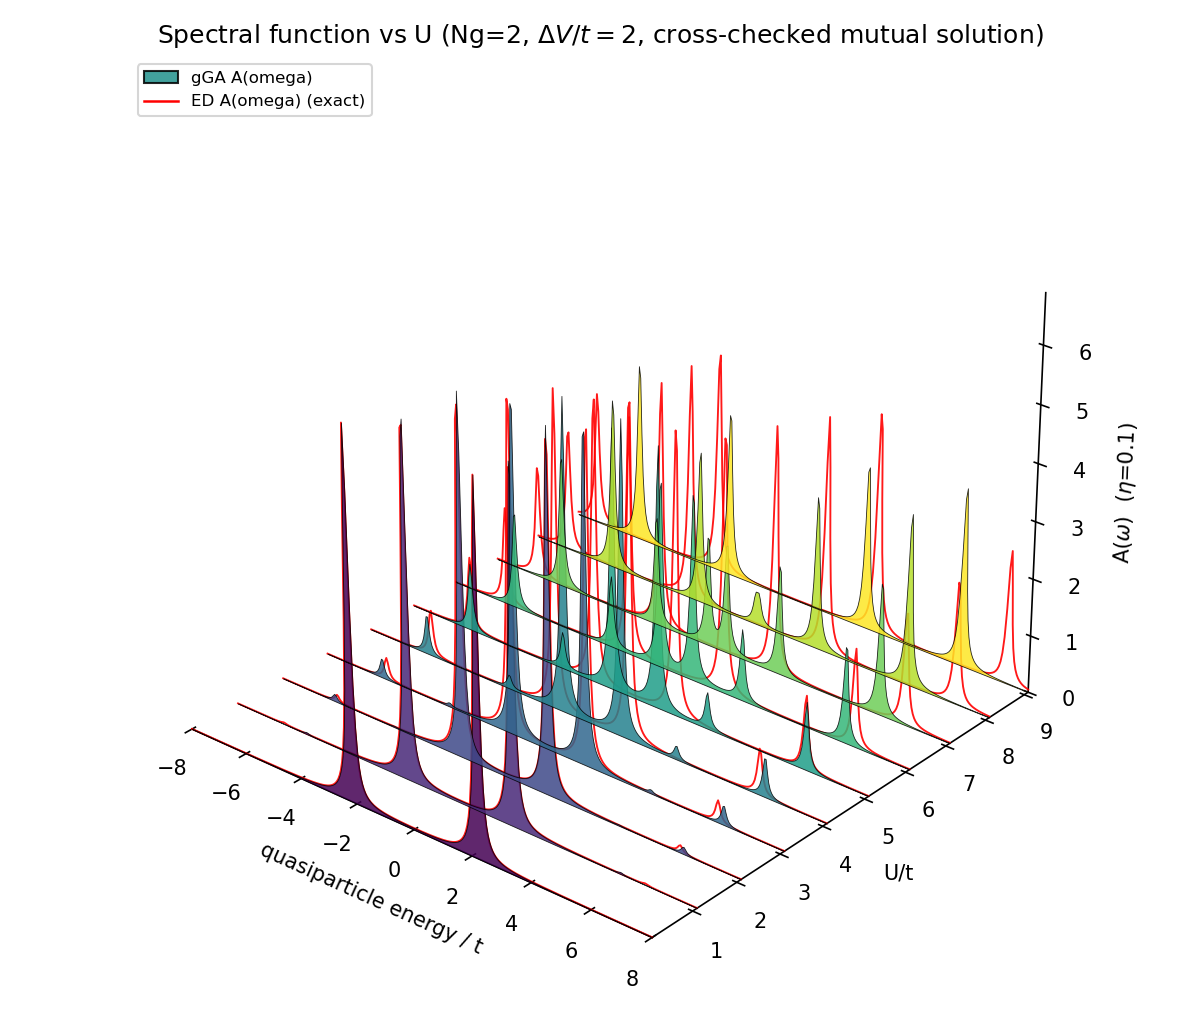
\includegraphics[width=\textwidth]{../scan_ng2_dV2_confirmed/eqp_vs_U_3d.png}
    \caption{$\dV=2$}
  \end{subfigure}
  \caption{$\Ng=2$: quasiparticle spectrum vs. $U/t$, 3D view.}
  \label{fig:ng2_3d}
\end{figure}

\subsection{Spectral function movies}

\begin{itemize}[nosep]
  \item $\dV=0$: \href{run:../scan_ng2_not_imp/A_omega_vs_U.mp4}{\texttt{scan\_ng2\_not\_imp/A\_omega\_vs\_U.mp4}}
  \item $\dV=2$: \href{run:../scan_ng2_dV2_confirmed/A_omega_vs_U.mp4}{\texttt{scan\_ng2\_dV2\_confirmed/A\_omega\_vs\_U.mp4}}
\end{itemize}
\noindent (Links open the file with the PDF viewer's associated application;
if the viewer does not support \texttt{run:} links, open the path directly.)

%=====================================================================
\section{\texorpdfstring{$\Ng=4$}{Ng=4}}
\label{sec:ng4}

\subsection{Total energy vs. \texorpdfstring{$U/t$}{U/t}}

\begin{figure}[H]
  \centering
  \begin{subfigure}[b]{0.48\textwidth}
    \centering
    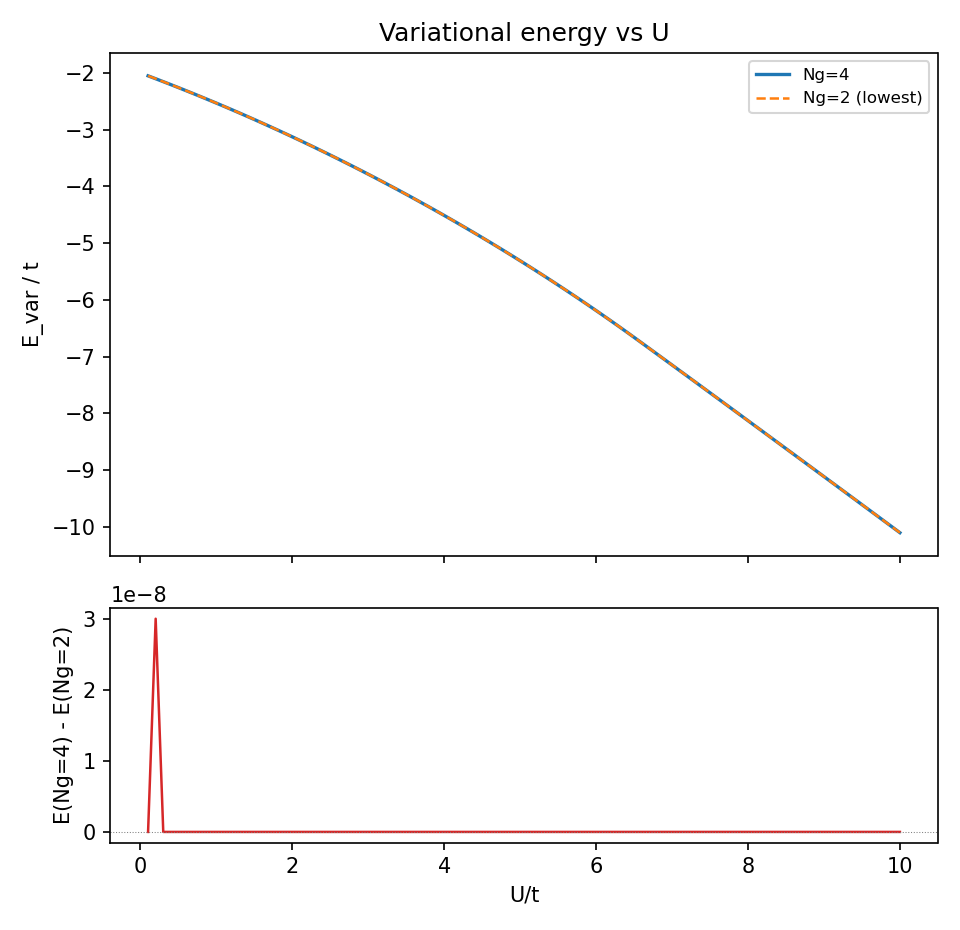
\includegraphics[width=\textwidth]{../scan_ng4_not_imp/E_vs_U.png}
    \caption{$\dV=0$}
  \end{subfigure}
  \hfill
  \begin{subfigure}[b]{0.48\textwidth}
    \centering
    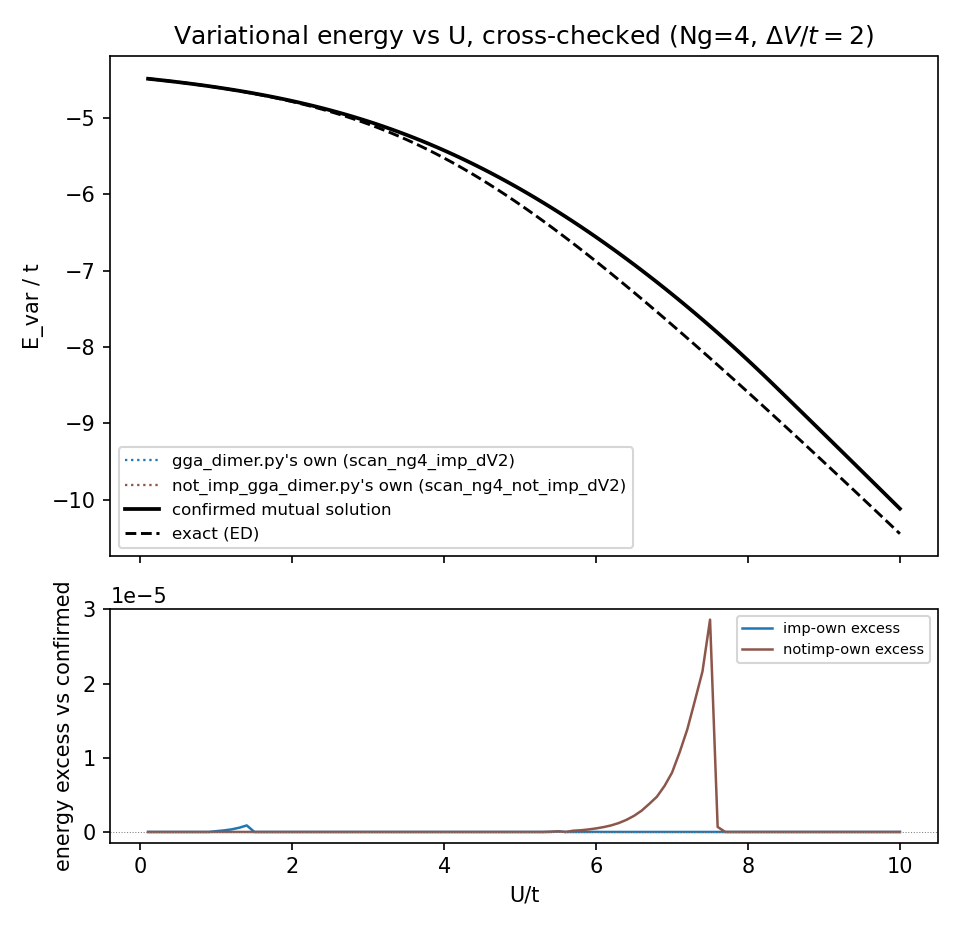
\includegraphics[width=\textwidth]{../scan_ng4_dV2_confirmed/E_vs_U.png}
    \caption{$\dV=2$}
  \end{subfigure}
  \caption{$\Ng=4$: total energy $E_{\rm var}/t$ vs. $U/t$. The $\dV=0$ panel
  also reports $E(\Ng=4)-E(\Ng=2)$ (see Section~\ref{sec:discussion}).}
  \label{fig:ng4_E}
\end{figure}

\subsection{Quasiparticle spectrum: 3D view}

\begin{figure}[H]
  \centering
  \begin{subfigure}[b]{0.48\textwidth}
    \centering
    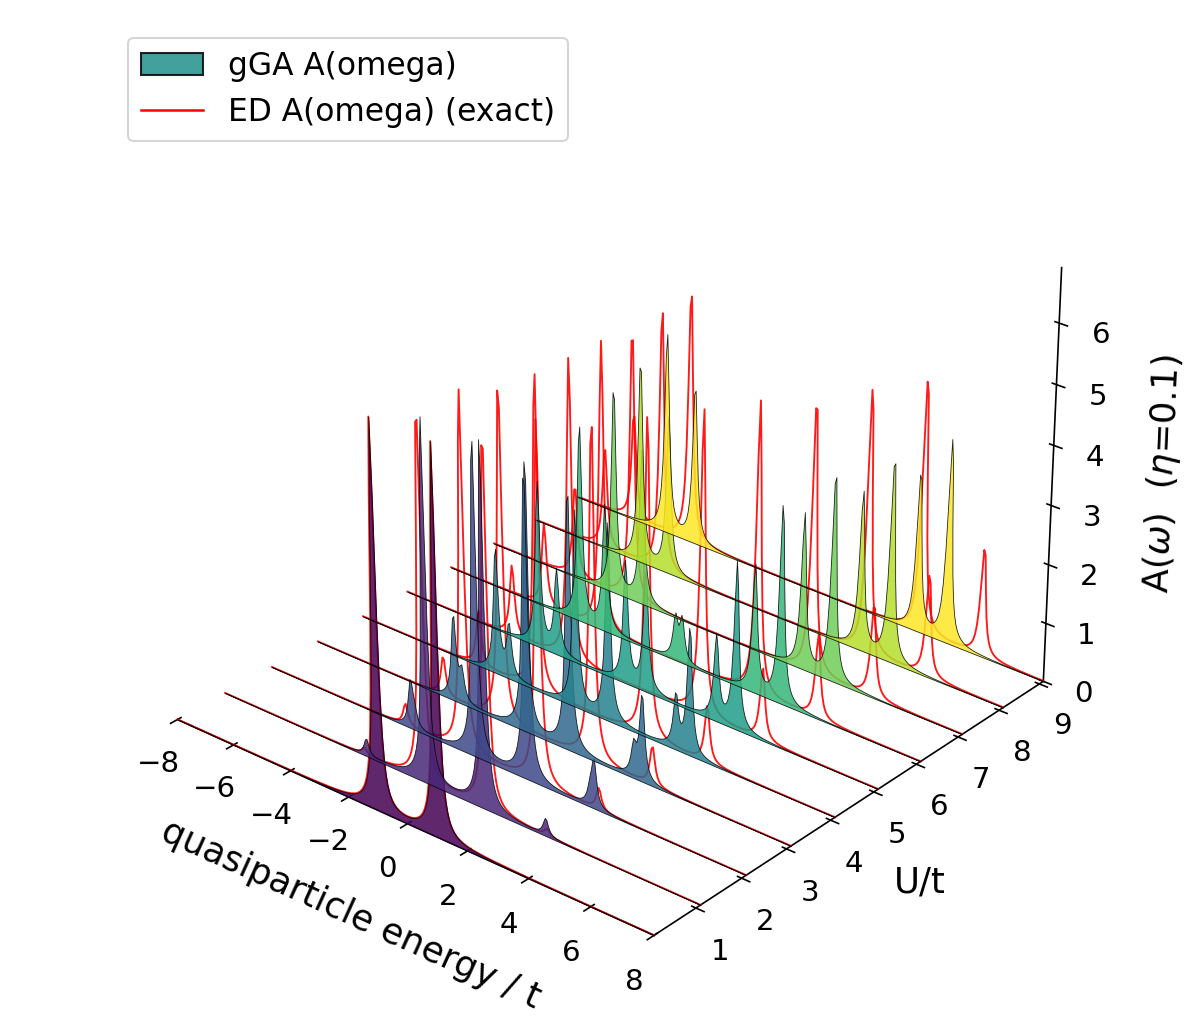
\includegraphics[width=\textwidth]{../scan_ng4_not_imp/eqp_vs_U_3d.png}
    \caption{$\dV=0$}
  \end{subfigure}
  \hfill
  \begin{subfigure}[b]{0.48\textwidth}
    \centering
    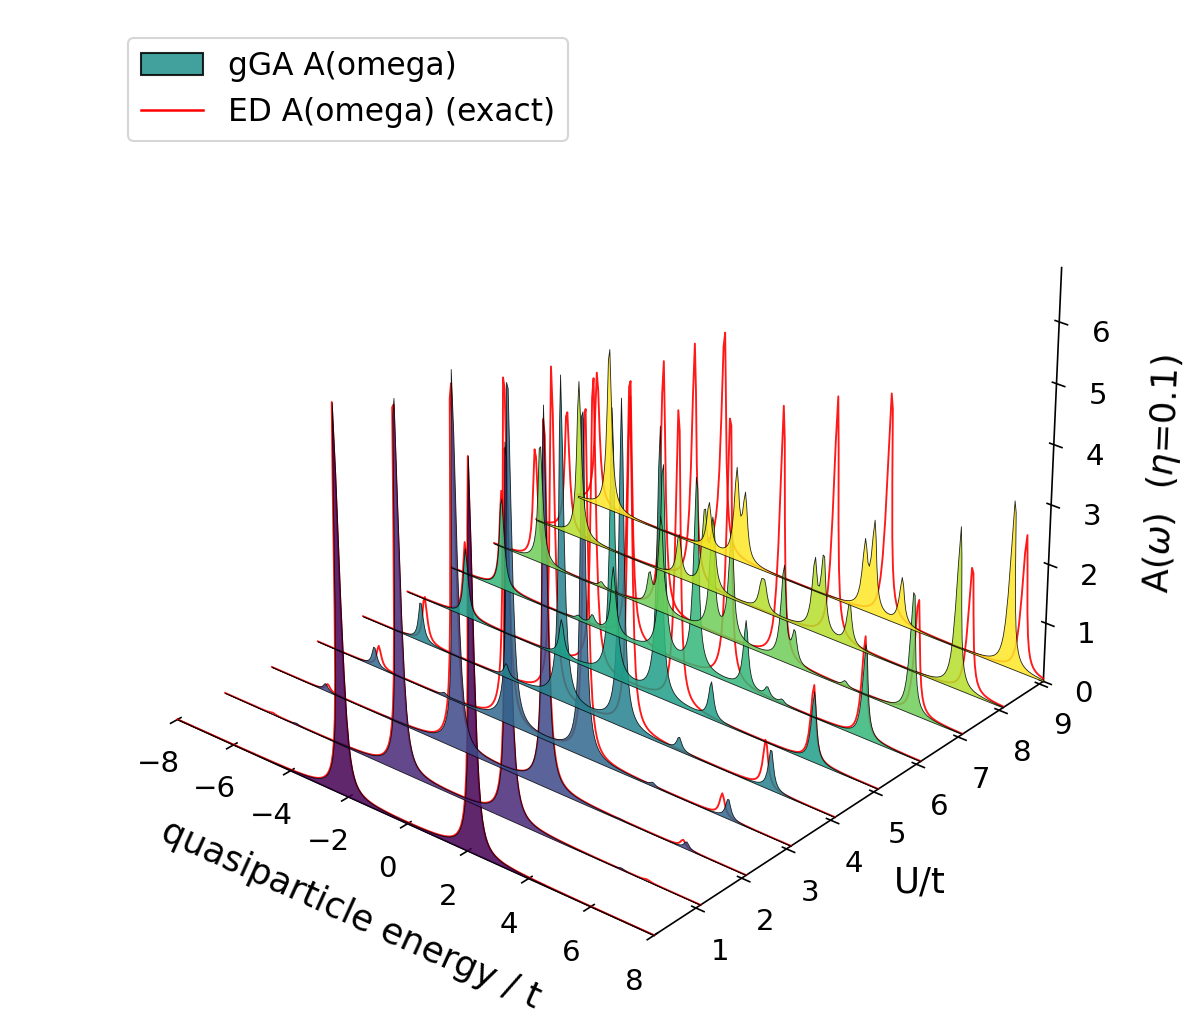
\includegraphics[width=\textwidth]{../scan_ng4_dV2_confirmed/eqp_vs_U_3d.png}
    \caption{$\dV=2$}
  \end{subfigure}
  \caption{$\Ng=4$: quasiparticle spectrum vs. $U/t$, 3D view. The larger ghost
  multiplicity doubles the number of quasiparticle branches compared to
  Figure~\ref{fig:ng2_3d}.}
  \label{fig:ng4_3d}
\end{figure}

\subsection{Spectral function movies}

\begin{itemize}[nosep]
  \item $\dV=0$: \href{run:../scan_ng4_not_imp/A_omega_vs_U.mp4}{\texttt{scan\_ng4\_not\_imp/A\_omega\_vs\_U.mp4}}
  \item $\dV=2$: \href{run:../scan_ng4_dV2_confirmed/A_omega_vs_U.mp4}{\texttt{scan\_ng4\_dV2\_confirmed/A\_omega\_vs\_U.mp4}}
\end{itemize}

%=====================================================================
\section{Discussion: \texorpdfstring{$\dV=0$}{dV=0} vs. \texorpdfstring{$\dV=2$}{dV=2}}
\label{sec:discussion}

\paragraph{Weak coupling: $\dV$ dominates.}
At small $U/t$ the two scans differ substantially. At $U/t=0.1$,
$E_{\rm var}/t = -2.0503$ for $\dV=0$ but $-4.4823$ for $\dV=2$ (both $\Ng$).
This is the expected $U\to0$ limit: with $\dV=0$ the dimer's noninteracting
energy is $-2t=-2$ plus a small $O(U)$ correction, while at $\dV=2$ the
site-splitting opens a one-body level gap and the $U\to0$ energy approaches
the closed form $E=-2\sqrt{t^2+\dV^2}=-2\sqrt{5}\approx-4.472$ (see
\texttt{project\_deltaV\_gga} validation). The gap between the two curves is
largest here, $\Delta E \approx 2.43$, because $\dV$ acts as an unscreened
one-body potential that the (still weak) correlations barely renormalize.

\paragraph{Strong coupling: the curves converge.}
As $U/t$ grows the two energies draw close together: at $U/t=10$,
$E_{\rm var}/t = -10.101$ ($\dV=0$) vs. $-10.120$ ($\dV=2$), a difference of
only $\approx 0.02$ -- two orders of magnitude smaller than at weak coupling.
In the Mott-like regime the total energy is governed almost entirely by $U$
(both sites approach single occupancy), and the fixed $\dV=2$ site-splitting
becomes a small perturbation on top of the dominant Hubbard physics. The
quasiparticle spectra (3D plots, Figs.~\ref{fig:ng2_3d}, \ref{fig:ng4_3d}) show
the same trend: the $\dV=2$ branches, well separated at small $U$, bunch
together with the $\dV=0$-like structure as $U/t$ increases.

\paragraph{Branch structure.}
At $\dV=0$ the lowest-energy solution alternates between ``forward'' and
``backward''-seeded branches as $U/t$ is swept (see
\texttt{scan\_ng2\_not\_imp/lowest\_energy.txt}), reflecting a near
degeneracy between the two sweep directions that the scan resolves by keeping
the lower of the two at each $U$. At $\dV=2$ this degeneracy is lifted by the
site-splitting itself, and the ``confirmed'' scans instead report a single
branch cross-checked between the impurity-problem and direct-minimization
solvers. The $\dV=2$ quasiparticle energies show a sharp rearrangement between
$U/t=0.6$ and $U/t=0.7$ (e.g.\ $\Ng=2$: $\epsilon^{qp}\approx-2.00\to-3.12$),
visible as a kink in the 3D plots; this is the level crossing where the
$\dV$-induced one-body gap stops being the dominant scale and the Hubbard
repulsion takes over.

\paragraph{Ghost multiplicity ($\Ng=2$ vs. $\Ng=4$).}
At both $\dV=0$ and $\dV=2$, doubling the ghost multiplicity from $\Ng=2$ to
$\Ng=4$ leaves the lowest variational energy numerically unchanged over the
whole scanned range: \texttt{scan\_ng4\_not\_imp/summary.txt} reports
$E(\Ng{=}4)-E(\Ng{=}2)=0$ to the printed precision at essentially every $U/t$
(largest deviation $\sim3\times10^{-8}$, at the level of solver tolerance), and
comparing \texttt{scan\_ng2\_dV2\_confirmed/lowest\_energy.txt} against
\texttt{scan\_ng4\_dV2\_confirmed/lowest\_energy.txt} shows the same agreement
at $\dV=2$ (e.g.\ $U/t=1.0$: $-4.593786$ vs.\ $-4.593786$). The extra ghost
degrees of freedom introduced at $\Ng=4$ therefore stay energetically inert
for this dimer at both values of $\dV$ in this $U$ range -- consistent with
the known $\Ng\ge2$ ``sleeping ghost'' caveat (\texttt{project\_deltaV\_gga}):
the additional branches exist in the quasiparticle spectrum (compare
Figs.~\ref{fig:ng2_3d} and \ref{fig:ng4_3d}, which show twice as many
$\epsilon^{qp}_n$ branches at $\Ng=4$) but do not lower the ground-state
energy below what $\Ng=2$ already finds.

\end{document}
